\chapter{Counterfactual Reasoning: COMING SOON}
\label{ch-counterf}
This chapter is mostly based on 
Ref.\cite{pearl-2019review}, a 2019
 review of causality by Pearl.


According to 
Judea Pearl,
there are 3 rungs in the
ladder of causal AI.
These are\footnote{This is my
own version of them. They differ 
slightly from Pearl's.  By now
you probably realize 
from reading
this book that I am a compulsive taylor
who can't resist  
altering the clothes I am gifted  so that they fit
me comfortably.}
\begin{enumerate}
\item
{\bf Dumb Observation:} Collecting 
data
and fitting curves to it,
without any plan 
designed to
investigate Nature's 
causal connections.
\item {\bf Doing causal
experiments:} 
Doing experiments 
consciously designed to
elucidate
Nature's causal connections.
Even cats do this!, but current AI doesn't.
\item {\bf Counterfactual reasoning:}
Imagining gedanken experiments
to further understand
Nature's causal connections,
and to decide what future
courses of action are
more likely to succeed,
even if there is zero
prior data for 
those courses of action.
This might be possible if there
is some similar
data that can be transported
(transplanted, applied)
to the situation of
interest--what we call
an analogy.
\end{enumerate}
Chapter \ref{ch-mp}
on message passing
is about rung 1.
Chapter \ref{chap-do-calc}
on do-calculus is about rung 2.
This chapter is dedicated to rung 3.

This chapter
assumes that the reader
has read
Chapter \ref{chap-do-calc}
on do-calculus.
This chapter also 
assumes that the reader has read 
Chapter \ref{ch-linear-sys}  
on LDEN (linear 
deterministic systems
with external noise).


\begin{figure}[h!]
\centering
\includegraphics[width=3in]
{counterf/rho-kappa.png}
\caption{Action
of operator $\rho_{\rvx=5}$
on node $\rvx$
and of operator 
$\kappa_{\rvx\rarrow \rvb}(5)$
on arrow $\rvx\rarrow \rvb$.} 
\label{fig-rho-kappa}
\end{figure}

\hrule
Let
us repeat
Eqs.(\ref{eq-nonlinear-pa-tpm})
and
(\ref{eq-pa-nonlinear-struc})
from Chapter \ref{ch-linear-sys}:


\beq\color{blue}
P(x_i|x_{<i}, u_i)=
\indi(
x_i=f_i(x_{<i}, u_i))
\;,
\label{eq-nonlinear-pa-tpm-copy}
\eeq

\beq
\rvx_i=f_i(\rvx_{<i}, \rvu_i)
\;,
\label{eq-pa-nonlinear-struc-copy}
\eeq
for $i=0, 1, \ldots, nx-1$.
These equations
are the TPMs and
structural equations
for a 
fully connected, non-linear DEN diagram.
For a non-fully connected 
diagram, 
\begin{itemize}
\item
replace the multinode $x_{<i}$
by a subset of itself,
in 
Eqs.(\ref{eq-nonlinear-pa-tpm-copy})
and (\ref{eq-pa-nonlinear-struc-copy})
,
and
\item
delete
the corresponding arrows
from the graph.
\end{itemize}


\hrule\noindent{\bf Intervention (do operation)
$\rho_{\rva=a}$  for LDEN diagram}.



\beq
\rvx=A\rvx +\rvu
\eeq

\beq
\rvx=(1-A)^{-1}\rvu
\eeq

\beq
\rvx_i = x_i(\rvu.)
\eeq 


Let $\pi_\rva$
be an $nx\times nx$ matrix with all entries equal
to  zero
except the $(i,i)$ entry, which is 1, 
where 
$i$  is such that $\rvx_i=\rva$.

\beq
(\pi_\rva)_{i,j}= \indi(i=j, \rva=\rvx_i)
\eeq

Let

\beq
\pi_{!\rva}=1-\pi_\rva
\eeq

\beq
A^*=\pi_{!\rva} A +a\pi_\rva
\eeq

\beq
\rvu_{!\rva}=\pi_{!\rva} \rvu
\eeq

\beq
\rvx^*= A^* \rvx^* + \rvu_{!\rva}
\eeq

\beq
\rvx^*=(1-A^*)^{-1} \rvu_{!\rva}
\eeq



\beq
\rvx^*_i=x^*_i(\pi_{!\rva}\rvu,a)
\eeq

\hrule
For any bnet,

\beq
P(\rvy=y|\rvx=x)
=
P_{G}(\rvy=y|\rvx=x)
\eeq

\beq
P(\rvy=y|\rho\rvx=x)
=
P_{\rho_{\rvx=x}G}(\rvy=y)
\eeq


\begin{claim}
For a non-linear DEN diagram,



\beq
P(y|\rho\rvx=x)=
E\left[
\delta[y, y(\pi_{!\rvx}\rvu,x)]\right]
\;.
\eeq
\end{claim}
\proof
\beqa
P(\rvy=y|\rho\rvx=x)
&=&
P_{\rho_{\rvx=x}G}(\rvy=y)
\\
&=&\sum_{\pi_{!\rvx}u}P(\pi_{!\rvx}u)
P_{\rho_{\rvx=x}G}
(\rvy=y|\pi_{!\rvx}u)
\\
&=&\sum_{\pi_{!\rvx}u}P(\pi_{!\rvx}u)
\delta[y, y(\pi_{!\rvx}u,x)]
\\
&=&
E_{\pi_{!\rvx}\rvu}
[\delta[y, y(\pi_{!\rvx}u, x)]]
\\
&=&
E[\delta[y,y(\pi_{!\rvx}\rvu, x)]]
\eeqa
\qed

\begin{claim}
For a nonlinear DEN diagram,

\beq
E[\rvy|\rho \rvx=x]=
E[y(\pi_{!\rvx}\rvu, x)]
\;.
\eeq
\end{claim}
\proof

\beqa
E[\rvy|\rho \rvx=x]
&=&
\sum_{y}
yP(\rvy=y|\rho\rvx=x)
\\
&=&
\sum_{y}
yE[
\delta[y, y(\pi_{!\rvx}u,x)]]
\\
&=&
E[y(\pi_{!\rvx}\rvu, x)]
\eeqa
\qed


For any bnet
\beqa
P(y|\rho\rvx=x, z)&=&
\frac{P(y, z|\rho\rvx=x)}
{P(z|\rho\rvx=x)}
=
P_{\rho_{\rvx=x}G}(y|x, z)
\eeqa

For a nonlinear DEN diagram,
\beq
P(y, z|\rho\rvx=x)
=
\sum_{\pi_{!\rvx}u}P(\pi_{!\rvx}u)
\delta[y, y(\pi_{!\rvx}u,x)]
\delta[z, z(\pi_{!\rvx}u,x)]
\eeq

\beq
P(z|\rho\rvx=x)=
\sum_{\pi_{!\rvx}u}P(\pi_{!\rvx}u)
\delta[z, z(\pi_{!\rvx}u,x)]
\;.
\eeq

\section*{Mediation Analysis}


\begin{figure}[h!]
$$\xymatrix{
\rvu_\rvt\ar[dd]
&\rvu_\rvm\ar[d]
&\rvu_\rvy\ar[dd]
\\
&\rvm\ar[rd]
\\
\rvt\ar[ru]\ar[rr]&&\rvy
\\
&G
}
\;\;\;\;\;\;\;\;\;\;\;\;
\xymatrix{
\rvu_\rvt\ar[dd]\ar@/^2pc/@{<-->}[r]
&\rvu_\rvm\ar[d]\ar@/^2pc/@{<-->}[r]
&\rvu_\rvy\ar[dd]
\\
&\rvm\ar[rd]
\\
\rvt\ar[ru]\ar[rr]&&\rvy
\\
&G^*
}$$
\caption{Graphs $G$ and $G^*$
are used to 
discuss mediation.}
\label{fig-mediation-bnets}
\end{figure}
\beqa
\rvt&=&f_\rvt(\rvu_\rvt)
\\
\rvm&=&f_\rvm(\rvt, \rvu_\rvm)
\\
\rvy&=&f_\rvy(\rvt, \rvm, \rvu_\rvy)
\eeqa

$\rho_{\rvt=5}G$
\beqa
\rvt&=&5
\\
\rvm&=&f_\rvm(\rvt, \rvu_\rvm)
\\
\rvy&=&f_\rvy(\rvt, \rvm, \rvu_\rvy)
\eeqa

$\kappa_{\rvt\rarrow\rvm}(5)G$
\beqa
\rvt&=&f_\rvt(\rvu_\rvt)
\\
\rvm&=&f_\rvm(5, \rvu_\rvm)
\\
\rvy&=&f_\rvy(\rvt, \rvm, \rvu_\rvy)
\eeqa

\beq
\rvy=f_\rvy(f_\rvt(u_\rvt), f_\rvm(\rvu_\rvt, \rvu_m))
\eeq



\begin{figure}[h!]
\centering
\begin{tabular}{m{6cm}m{6cm}}
$
\xymatrix{
\rvu_\rvt
&\rvu_\rvm\ar[d]
&\rvu_\rvy\ar[dd]
\\
&\rvm\ar[rd]
\\
\rvt=t\ar[ru]
\ar[rr]&&\rvy
}$
&
$
\xymatrix{
\rvu_\rvt
&\rvu_\rvm
&\rvu_\rvy\ar[dd]
\\
&\rvm=m\ar[rd]
\\
\rvt=t
\ar[rr]&&\rvy
}$
\\
$\;\;\;\;\;\;\;\;
\rho_{\rvt=t}G$
&
$\;\;\;\;\;\;\;\;
\rho_{\rvt=t}\rho_{\rvm=m}G$
\end{tabular}
\label{fig-mediation-rho}
\caption{Graph $G$
of Fig.\ref{fig-mediation-bnets}
with do operator $\rho$ applied to nodes
$\rvt$ and $(\rvt, \rvm)$.}
\end{figure}
Total Effect (TE),
Controlled Direct Effect (CDE)
\beqa
TE&=& E[
\rvy_{\rho_{\rvt=1}G}
-\rvy_{\rho_{\rvt=0}G}
]
\\
CDE(m)&=&
E[
\rvy_{\rho_{\rvt=1}\rho_{\rvm=m}G}
-\rvy_{\rho_{\rvt=0}\rho_{ \rvm=m}G}
]
\eeqa
\hrule

\begin{figure}[h!]
\centering
\begin{tabular}{m{4cm}m{3cm}}
$
\kappa_{\rvt\rarrow\rvy}(a)
\kappa_{\rvt\rarrow\rvm}(b)G
=$
&
$\xymatrix{
\rvu_\rvt\ar[dd]
&\rvu_\rvm\ar[d]
&\rvu_\rvy\ar[dd]
\\
&\rvm\ar[rd]
\\
\rvt\ar[ru]^{\kappa(b)}
\ar[rr]^{\kappa(a)}&&\rvy
}$
\end{tabular}
\label{fig-mediation-kappa}
\caption{
Graph $G$
of Fig.\ref{fig-mediation-bnets}
with counterfactual
 operator $\kappa$
 applied to arrows
$\rvt\rarrow\rvm$ and $\rvt\rarrow\rvy$.}
\end{figure}


\beq
E^{b}_{a}=
 E[
\rvy_{\kappa_{\rvt\rarrow\rvy}(a)
\kappa_{\rvt\rarrow\rvm}(b)G}
]
\eeq



Natural Direct Effect (NDE),
Natural Indirect Effect (NIE)
\beqa
NDE
&=&E_1^0 - E_0^0
\\
NIE(t)
&=&E_t^1 - E_t^0
\eeqa


\beqa
NDE+NIE(1)&=&(E_1^0-E_0^0)+(E_1^1 - E_1^0)
\\
&=&E_1^1-E_0^0
\\
&=&
TE
\eeqa


